        \clearpage
        \begin{figure*}[ht]
            \pdfbookmark[2]{ID 06}{figure_id_06}
        	\centering
            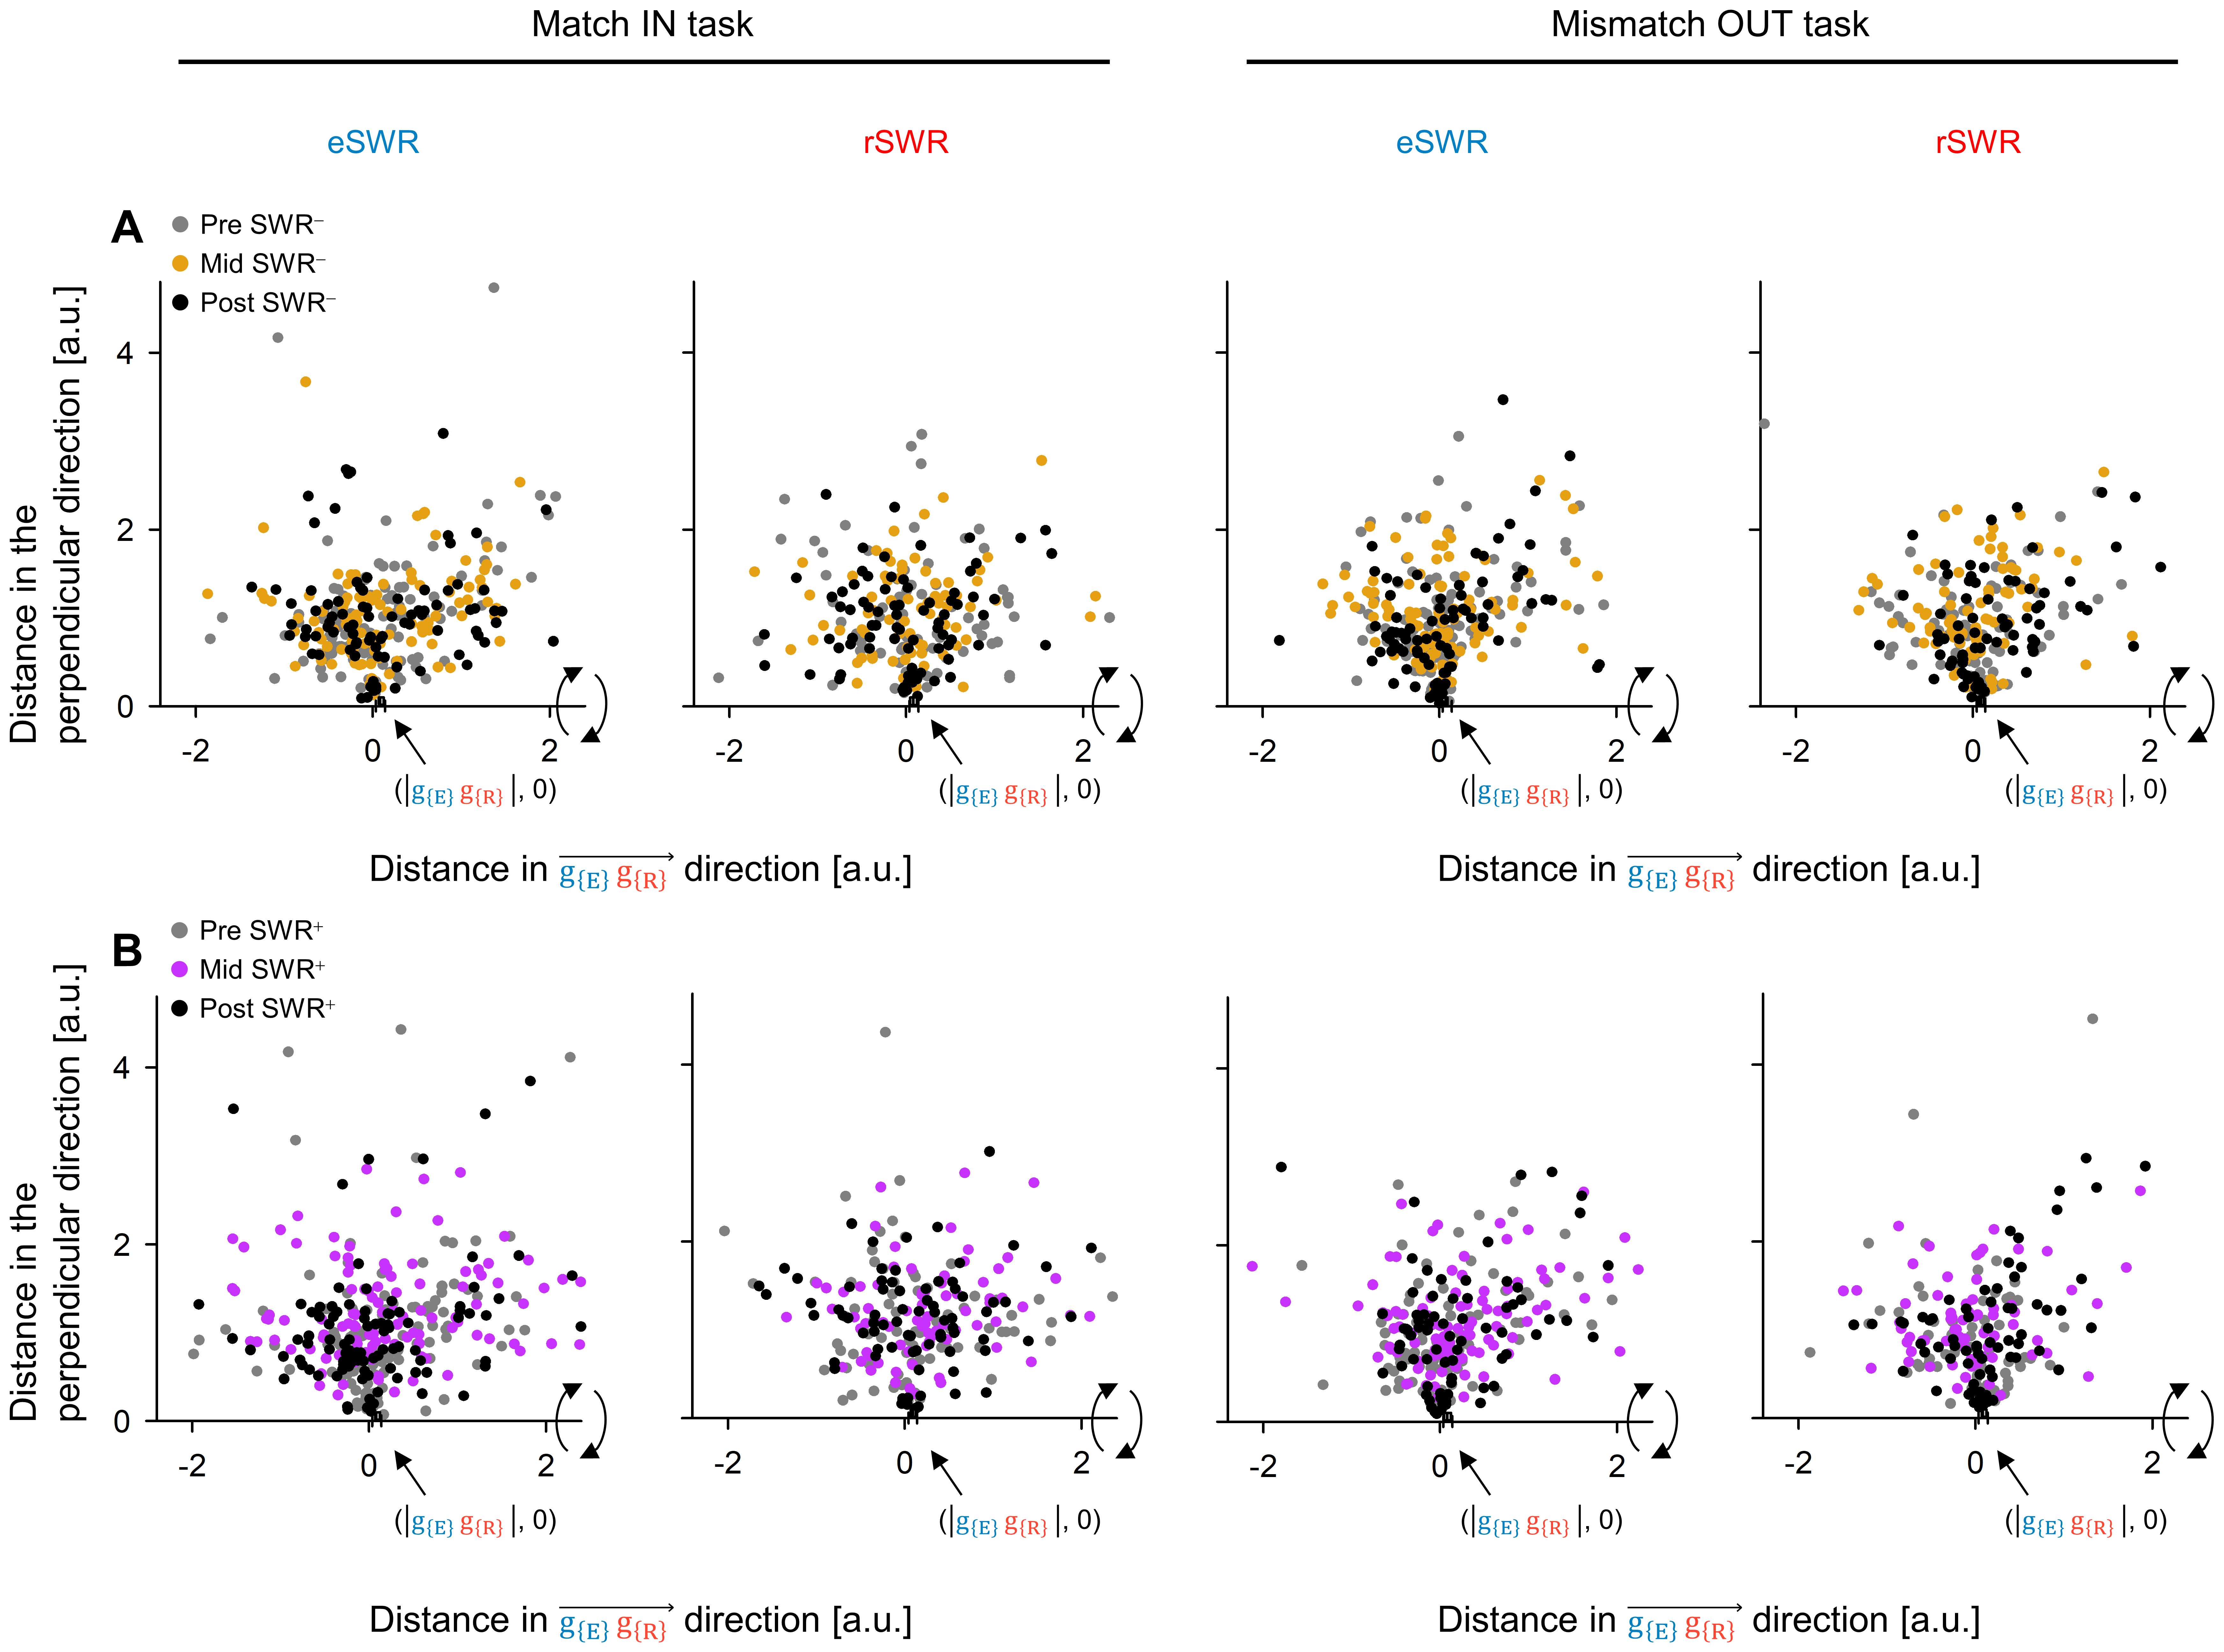
\includegraphics[width=]{./src/figures/.png/Figure_ID_06.png}
        	\caption{\textbf{Visualization of Neural Trajectories during Sharp-Wave Ripple Events in Two-Dimensional Space}
\smallskip
\\
The panels portray hippocampal neural trajectories (NTs) during sharp-wave ripple (SWR) events, projected onto two-dimensional spaces. \textbf{\textit{A.}} Displays the hippocampal NTs as point clouds during pre-SWR$^-$ (in gray), mid-SWR$^-$ (in yellow), and post-SWR$^-$ (in black). \textbf{\textit{B.}} Presents the comparable depiction for SWR$^+$ instead of SWR$^-$. The projection was undertaken as follows: Firstly, a linear transformation set $\mathrm{g_{E}}$ at the origin point $O$ (0,0), and $\mathrm{g_{R}}$ at ($\lVert \mathrm{g_{E}g_{R}} \rVert$, 0). Subsequently, the point cloud was rotated around the $\mathrm{g_{E}g_{R}}$ axis (akin to the x-axis), adjusting it to two-dimensional spaces. As such, in these two-dimensional spaces, the distances from point $O$ and the angles for the $\mathrm{g_{E}g_{R}}$ axis are preserved identically as in the original three-dimensional spaces generated by Gaussian Process Factor Analysis (GPFA). Abbreviations: SWR denotes sharp-wave ripple events; encoding sharp-wave ripple (eSWR) refers to SWR during the encoding phase; retrieval sharp-wave ripple (rSWR) indicates SWR during the retrieval phase; SWR$^+$ characterizes a SWR event; SWR$^-$ designates control events for SWR$^+$; pre-SWR, mid-SWR, or post-SWR define the time intervals from $-800$ to $-250$ ms, from $-250$ to $+250$ ms, or from $+250$ to $+800$ ms from the center of SWR, respectively.
}
        	\label{fig:06}
        \end{figure*}
